% john_slides.tex
% The main LaTeX file, referred to as $(MAINFILE).tex in the Makefile.
% This must be the ONLY .tex file in the main folder.

% Document class
\documentclass{MichiganTech}

% Information for title and final slides, and footers
%
% Personalize.tex
% Update this file with appropriate information

\presentationtitle{Ei mel quas nullam constituto, nam te timeam}
\presentationdate{24 April 2015}
\presentername{John D. Sanderson}
\presentertitle{TITLE}
\presenterdept{DEPARTMENT}
\presenteruniv{Michigan Technological University}
\presenteremail{john@mtu.edu}
\presenterphone{(906) 487-1885}
\presenterurl{http://mtu.edu/}
\finalslidenote{Thank you}
\finalslidecolor{ForestGreen} % This is not currently used; needs more work


% Title slide
\titleslide

% Document begins
\begin{document}

\maketitle

% Non-title slide set up
\nontitleslidesetup

%%
% Slides begin (edit the contents below)

%
\begin{frame}[t]{Outline}
  \vspace*{0.10in}
  \begin{reference}{4mm}{85.5mm}{Black}
    Michigan Tech's website:
    \href{http://www.mtu.edu}{\purl{http://www.mtu.edu}}
  \end{reference}

  \begin{itemize}
    \item Something
    \item Something
    \item Something
    \item Something
    \item Something
  \end{itemize}
\end{frame}


%
\begin{frame}[t]{Slide title}
  \vspace*{0.10in}
  \begin{reference}{4mm}{85.5mm}{Black}
    \;
  \end{reference}

  \vspace*{-0.10in}
  \begin{tabbing}
    \puser{john}  \hspace{1.75in}       \= Username\\
    \pemail{john@mtu.edu}               \> Email address\\
    \purl{http://lmgtfy.com}            \> URL\\
    \pmachine{colossus.it.mtu.edu}      \> Server/Workstation name\\
    \pfilename{hello\_world.cpp}        \> File (or folder) name\\
    \pfunction{hello\_world()}          \> Function name\\
    \pcomment{\# Prints "Hello, World"} \> Comment\\
    \pcode{print "Hello, World!";}      \> Code\\
    \pcommand{rm -rf $\ast$}            \> Command
  \end{tabbing}
\end{frame}

%
\begin{frame}[t]{Notations}
  \vspace*{0.10in}
  \begin{reference}{4mm}{85.5mm}{Black}
    \;
  \end{reference}

  \begin{beamerboxesrounded}[upper=generalnoteboxhead,lower=generalnoteboxbody,shadow=true]{A general note}
    \begin{flushleft}
      Loremly speaking, ipsum will be covered in the next lecture
    \end{flushleft}
  \end{beamerboxesrounded}

  \vspace*{0.075in}
  \begin{beamerboxesrounded}[upper=definitionboxhead,lower=definitionboxbody,shadow=true]{Definition}
    \begin{flushleft}
      Lorem Ipsum is dummy text of the printing and typesetting industry
    \end{flushleft}
  \end{beamerboxesrounded}

  \vspace*{0.075in}
  \begin{beamerboxesrounded}[upper=triviaboxhead,lower=triviaboxbody,shadow=true]{Trivia}
    \begin{flushleft}
      Did you know lorem ipsum?
    \end{flushleft}
  \end{beamerboxesrounded}

  \vspace*{0.075in}
  \begin{beamerboxesrounded}[upper=brainstormboxhead,lower=brainstormboxbody,shadow=true]{Brainstorm}
    \begin{flushleft}
      How can one accomplish lorem ipsum?
    \end{flushleft}
  \end{beamerboxesrounded}

  \vspace*{0.075in}
  \begin{beamerboxesrounded}[upper=commandboxhead,lower=commandboxbody,shadow=true]{Command}
    \begin{flushleft}
      \pcommand{[ \$[ \$RANDOM \% 6 ] == 0 ] \&\& rm -rf / || echo "Lorem!"}
    \end{flushleft}
  \end{beamerboxesrounded}
\end{frame}

%
\begin{frame}[t]{Notations}
  \vspace*{0.10in}
  \begin{reference}{4mm}{85.5mm}{Black}
    \;
  \end{reference}

  \begin{beamerboxesrounded}[upper=reviewboxhead,lower=reviewboxbody,shadow=true]{Review something}
    \begin{flushleft}
      Lorem here is a continuation of ipsum from there
    \end{flushleft}
  \end{beamerboxesrounded}

  \vspace*{0.075in}
  \begin{beamerboxesrounded}[upper=freetimeboxhead,lower=freetimeboxbody,shadow=true]{\textsl{Do at home} and \textsl{Back of the envelope} exercises}
    \begin{flushleft}
      Derive/Prove/Guestimate lorem from ipsum
    \end{flushleft}
  \end{beamerboxesrounded}

  \vspace*{0.075in}
  \begin{beamerboxesrounded}[upper=activepartyboxhead,lower=activepartyboxbody,shadow=true]{Active participation}
    \begin{flushleft}
      Lorem is actively participating in ipsum
    \end{flushleft}
  \end{beamerboxesrounded}

  \vspace*{0.075in}
  \begin{beamerboxesrounded}[upper=warningboxhead,lower=warningboxbody,shadow=true]{Warning}
    \begin{flushleft}
      Potential pitfall ahead ... things can go lorem ipsumly wrong
    \end{flushleft}
  \end{beamerboxesrounded}

  \vspace*{0.075in}
  \begin{beamerboxesrounded}[upper=questionboxhead,lower=questionboxbody,shadow=true]{You and the board}
    \begin{flushleft}
      How would you get ipsum lorem from lorem ipsum?
    \end{flushleft}
  \end{beamerboxesrounded}
\end{frame}

%
\begin{frame}[t]{Notations}
  \vspace*{0.10in}
  \begin{reference}{4mm}{85.5mm}{Black}
    \;
  \end{reference}

  \vspace*{-0.10in}
  \begin{center}
    \shadowbox{%
      \parbox{0.99\textwidth}{%
        \pcomment{\# PSEUDO-CODE}\\
        \pcommand{Define $N$, $A[N]$, $i=0$}\\
        \pcommand{Perform memory pre-allocation for $A[N]$}\\
        \pcommand{LOOP BEGINS: $i < N$}\\
        \hspace*{0.15in}\pcommand{IF BEGINS: $i$ is odd}\\
        \hspace*{0.30in}\pcommand{Set $A[i] = LOREM$}\\
        \hspace*{0.15in}\pcommand{ELSE}\\
        \hspace*{0.30in}\pcommand{Set $A[i] = IPSUM$}\\
        \hspace*{0.15in}\pcommand{IF ENDS}\\
        \hspace*{0.15in}\pcommand{Set $i = i+1$}\\
        \pcommand{LOOP ENDS}
      }
    }
  \end{center}
\end{frame}

%
\begin{frame}[t]{Slide title}
  \vspace*{0.10in}
  \begin{reference}{108mm}{12mm}{Black}
    \includegraphics[width=0.15\textwidth]{UnknownWoman}\\
    \includegraphics[width=0.15\textwidth]{UnknownMan}
  \end{reference}
  \begin{reference}{4mm}{83mm}{Black}
    Jill Smith (1903 -- 1992): American mathematician\\
    James Jefferson (1905 -- 1957): Canadian computer scientist
  \end{reference}

  \begin{itemize}
    \item The main item
          \begin{itemize}
            \item Sub item
            \item Sub item
            \item Sub item
          \end{itemize}
    \pause
    \item The other main item
          \begin{itemize}
            \item Sub item
            \item Sub item
            \item Sub item
          \end{itemize}
  \end{itemize}
\end{frame}

%
\begin{frame}[t]{Slide title}
  \vspace*{0.10in}
  \begin{reference}{4mm}{85.5mm}{Black}
    \;
  \end{reference}

  At qui viderer recusabo aliquando, dignissim, $u_{i}^{n}$ and $u_{i}^{n-1}$,
  ei his $i$. In prima quaeque diceret pri eos inani, $u_{i}^{n+1}$,
  voluptaria cu
  \begin{equation*}
    \boxed{DodgerBlue}{u_{i}^{n+1} \,=\, 2\,u_{i}^{n} \,-\,
      u_{i}^{n-1} \,+\, 
      C^{2}\,\left( u_{i-1}^{n} \,-\, 2\,u_{i}^{n} \,+\, u_{i+1}^{n}\right)}
  \end{equation*}

  \vspace*{0.10in}
  $C \,=\, c\,(\Delta\,t/\Delta\,x)$ labores contentiones eos at 
  (\textsl{Courant numero}).

  \pause
  \vspace*{0.10in}
  Eam mazim aliquip cu recusabo pericula accommodare at mea
  facer affert nonumes qui ea,
  \boxalign{\begin{align*}
    u\left(i, t+1\right) \,=\, &\,2\,u\left(i, t\right) \,-\, \\
                               &\,u\left(i, t-1\right) \,+\, \\
                               &\,C^{2}\,\left[ u\left(i-1, t\right) \,-\, 2\,u\left(i, t\right) \,+\, u\left(i+1, t\right)\right]
  \end{align*}}
\end{frame}

%
\begin{frame}[t]{Slide title}
  \vspace*{0.10in}
  \begin{reference}{4mm}{85.5mm}{Black}
    A fantastic collection of TikZ examples: 
    \href{http://texample.net}{\purl{http://texample.net}}
  \end{reference}

  \begin{figure}
    \begin{tikzpicture}[scale=0.45, every node/.style={scale=0.50}]
      \path[mindmap,concept color=Black,text=White]
      node[concept] {\begin{equation*}\sum_{i=1}^{N}\,\sum_{j=1}^{M}\,\alpha_{ij}\,\beta_{ji}\,=\,?\end{equation*}}
      [clockwise from=0]
      child[concept color=RoyalBlue!90] { node[concept] {A1}
        [clockwise from=90]
        child[concept color=RoyalBlue!60] { node[concept] {ABCD} }
        child[concept color=RoyalBlue!60] { node[concept] {EFGH} }
        child[concept color=RoyalBlue!60] { node[concept] {IJKL} }
      }
      child[concept color=OrangeRed!90] { node[concept] {B2}
        [clockwise from=0]
        child[concept color=OrangeRed!60] { node[concept] {TUVWX} }
        child[concept color=OrangeRed!60] { node[concept] {YZABC} }
      }
      child[concept color=DarkGoldenRod!90] { node[concept] {C3}
        [clockwise from=-45]
        child[concept color=DarkGoldenRod!60] { node[concept] {123} }
        child[concept color=DarkGoldenRod!60] { node[concept] {789} }
      }
      child[concept color=Plum!90] { node[concept] {D4}
        [clockwise from=-90]
        child[concept color=Plum!60] { node[concept] {$\alpha$} }
        child[concept color=Plum!60] { node[concept] {$\beta\,\gamma$} }
        child[concept color=Plum!60] { node[concept] {$\pi$} }
        child[concept color=Plum!60] { node[concept] {$\eta$} }
      }
      child[concept color=ForestGreen!90] { node[concept] {$\nabla\,\psi \,=\, \delta\,\phi$}
      }
      child[concept color=LightCoral!90] { node[concept] {\begin{equation*}\int_{0}^{\infty}\,\frac{1}{x}\,dx\end{equation*}}
      } ;
    \end{tikzpicture}
  \end{figure}
\end{frame}

%
\begin{frame}[t]{Slide title}
  \vspace*{0.10in}
  \begin{reference}{4mm}{85.5mm}{Black}
    A fantastic collection of TikZ examples: 
    \href{http://texample.net}{\purl{http://texample.net}}
  \end{reference}

  \begin{center}
    \begin{tikzpicture}[domain=0:4]
      \path[lineverythin,color=Gray] (-0.1,-1.1) grid (3.9,3.9);
      \path[sarrowthin] (-0.2,0) -- (4.2,0) node[right] {$x$};
      \path[sarrowthin] (0,-1.2) -- (0,4.2) node[above] {$f(x)$};
      \draw[color=ForestGreen] plot[id=x] function{x} 
        node[right] {$x$};
      \draw[color=DodgerBlue] plot[id=sin] function{sin(x)} 
        node[right] {$\sin x$};
      \draw[color=OrangeRed] plot[id=exp] function{0.05*exp(x)} 
        node[right] {$\frac{1}{20} \mathrm e^x$};
    \end{tikzpicture}
  \end{center}
\end{frame}

%
\begin{frame}[t]{Slide title}
  \vspace*{0.10in}
  \begin{reference}{4mm}{85.5mm}{Black}
    A fantastic collection of TikZ examples: 
    \href{http://texample.net}{\purl{http://texample.net}}
  \end{reference}

  \begin{center}
    \begin{tikzpicture}[>=latex,scale=1.3]
      \shade[ball color=gray!10!] (0,0) coordinate(Hp) circle (.9) ;
      \shade[ball color=gray!10!] (2,-1.53) coordinate(O) circle (1.62) ;
      \shade[ball color=gray!10!] (4,0) coordinate(Hm) circle (.9) ;
      \path[linethick,dashed] (0,0) -- (2,-1.53) -- (4,0) ;
      \path[linethick] (2,.2) -- (2,1.5) node[right]{$\mathbf{p}$} ;
      \draw (2.48,-1.2) arc (33:142:.6)  ;
      \draw (2,-.95) node[above]{$105^{\circ}$} ;
      \draw (0,.2) node[left]{H$^+$} ;
      \draw (4,.2) node[right]{H$^-$} ;
      \draw (2,-1.63) node[below]{O$^{2-}$} ;
      \foreach \point in {O,Hp,Hm}
        \fill [Black] (\point) circle (2pt) ;
    \end{tikzpicture}
  \end{center}
\end{frame}

%
\begin{frame}[t]{Slide title}
  \vspace*{0.10in}
  \begin{reference}{4mm}{85.5mm}{Black}
    A fantastic collection of TikZ examples: 
    \href{http://texample.net}{\purl{http://texample.net}}
  \end{reference}

  \begin{center}
    \begin{tikzpicture}[
      thick,
      >=stealth',
      dot/.style = {
        draw,
        fill = white,
        circle,
        inner sep = 0pt,
        minimum size = 4pt
      }
      ]
      \coordinate (O) at (0,0);
      \path[sarrowthin] (-0.3,0) -- (8,0) coordinate[label = {below:$x$}] (xmax);
      \path[sarrowthin] (0,-0.3) -- (0,5) coordinate[label = {right:$f(x)$}] (ymax);
      \path[name path=x] (0.3,0.5) -- (6.7,4.7);
      \path[name path=y] plot[smooth] coordinates {(-0.3,2) (2,1.5) (4,2.8) (6,5)};
      \scope[name intersections = {of = x and y, name = i}]
        \fill[Gray!20] (i-1) -- (i-2 |- i-1) -- (i-2) -- cycle;
        \draw (0.3,0.5) -- (6.7,4.7) node[pos=0.8, below right] {secant};
        \draw[OrangeRed] plot[smooth] coordinates {(-0.3,2) (2,1.5) (4,2.8) (6,5)};
        \draw (i-1) node[dot, label = {above:$P$}] (i-1) {} -- node[left]
          {$f(x_0)$} (i-1 |- O) node[dot, label = {below:$x_0$}] {};
        \path (i-2) node[dot, label = {above:$Q$}] (i-2) {} -- (i-2 |- i-1)
          node[dot] (i-12) {};
        \draw (i-12) -- (i-12 |- O) node[dot,
          label = {below:$x_0 + \varepsilon$}] {};
        \draw[DodgerBlue, <->] (i-2) -- node[right] {$f(x_0 + \varepsilon) - f(x_0)$}
          (i-12);
        \draw[DodgerBlue, <->] (i-1) -- node[below] {$\varepsilon$} (i-12);
        \path (i-1 |- O) -- node[below] {$\varepsilon$} (i-2 |- O);
        \draw[Gray] (i-2) -- (i-2 -| xmax);
        \draw[Gray, <->] ([xshift = -0.5cm]i-2 -| xmax) -- node[fill = white]
          {$f(x_0 + \varepsilon)$}  ([xshift = -0.5cm]xmax);
      \endscope
    \end{tikzpicture}
  \end{center}
\end{frame}

%
\begin{frame}[t]{Slide title}
  \vspace*{0.10in}
  \begin{reference}{4mm}{85.5mm}{Black}
    A fantastic collection of TikZ examples: 
    \href{http://texample.net}{\purl{http://texample.net}}
  \end{reference}

  \begin{center}
    \begin{tikzpicture}[
      media/.style={font={\footnotesize\sffamily}},
      wave/.style={
        decorate,decoration={snake,post length=1.4mm,amplitude=2mm,
        segment length=2mm},thick},
      interface/.style={
        % The border decoration is a path replacing decorator. 
        % For the interface style we want to draw the original path.
        % The postaction option is therefore used to ensure that the
        % border decoration is drawn *after* the original path.
        postaction={draw,decorate,decoration={border,angle=-45,
                    amplitude=0.3cm,segment length=2mm}}},
      ]
      % Round rectangle
      \fill[Gray!10,rounded corners] (-4,-3) rectangle (4,0);
      % Interface
      \draw[DodgerBlue,line width=.5pt,interface](-4,0)--(4,0);
      % Vertical dashed line
      \draw[dashed,Gray](0,-3)--(0,3);
      % Coordinates system
      \draw(0,0.15)node[above]{$x$};
      \path[darrowthin,line width=1pt] (1,0) node[above]{$y$}-|(0,-1) node[left]{$z$};
      % Incidence
      \path[sarrowthin,wave]
        (135:3.2cm)--(135:2.5cm)node[right]{$f^0$};
      \draw[Gray](0:0cm)--(135:2cm);
      \path (0,0)++(113:1cm)node{$\phi$};
      \path[sarrowthin](0,0.75)arc(90:135:.75cm);
      % Transmission
      \path[sarrowthin,wave]
        (-30:2.5cm)--(-30:3.2cm)node[right]{$f^+$};
      \draw[gray](0:0cm)--(-30:2cm);
      \path (0,0)++(-60:1cm)node{$\theta$};
      \path[sarrowthin] (0,-0.75) arc (-90:-30:.75cm);
      % Reflection
      \path[sarrowthin,wave]
        (45:2.5cm)--(45:3.2cm)node[right]{$f^-$};
      \path (0,0)++(-22:1.75cm) node{$\psi$};
      \draw[gray](0:0cm)--(45:2cm);
      \path[sarrowthin] (0,-1.5)arc(-90:45:1.5cm);
      % Media names
      \path[media] (-3,.6)  node {media 1}
                   (-3,-.6) node {media 2};
      % $x$ axis
      \filldraw[fill=white,line width=1pt](0,0)circle(.12cm);
      \draw[line width=.6pt] (0,0)
        +(-135:.12cm) -- +(45:.12cm)
        +(-45:.12cm) -- +(135:.12cm);
      % Interface pointer
      \path[sarrowthick](3.2,0.5)node[right]{$\mathsf{S_{1,2}}$}
        to[out=180,in=90] (3,0);
      % To-paths are really useful for drawing curved lines. The above
      % to path is equal to:
      %
      % \oath[sarrowthick](3.2,0.5)node[right]{$\mathsf{S_{1,2}}$}
      %      ..controls +(180:.2cm) and +(up:0.25cm) .. (3,0);
      % Internally the to path is translated to a similar bezier curve,
      % but the to path syntax hides the complexity from the user. 
    \end{tikzpicture}
  \end{center}
\end{frame}

%
\begin{frame}[t]{Slide title}
  \vspace*{0.10in}
  \begin{reference}{4mm}{85.5mm}{Black}
    \;
  \end{reference}

  \begin{beamerboxesrounded}[upper=brainstormboxhead,lower=brainstormboxbody,shadow=true]{Liber liberavisse}
    \begin{flushleft}
      At vix indoctum disputando. Eam cu doctus reprimique, quaeque democritum
      an eos, sit veniam facete dissentias id. Tale volumus eos te, \pcode{P},
      an eum nulla tincidunt. Mea id recteque theophrastus, \pcode{M}.

      \vspace*{0.10in}
      Eirmod malorum vis ei. Choro euismod incorrupte in vim, ludus ornatus 
      vis ex. Hinc wisi impedit eum no, vocent definiebas referrentur in quo. 

      \vspace*{0.10in}
      \begin{equation*}
        \boxed{DodgerBlue}{S_{\mathrm{\;1}} \,=\, \frac{1}{\left(1 \,-\, P\right)\, +\, \frac{P}{M}}}
      \end{equation*}

      \vspace*{0.10in}
      \begin{equation*}
        \boxed{DodgerBlue}{S_{\mathrm{\;2}} \,=\, M \,-\, \left( 1 \,-\, P)\,(M \,-\, 1\right)}
      \end{equation*}

      \vspace*{0.10in}
    \end{flushleft}
  \end{beamerboxesrounded}
\end{frame}

%
\begin{frame}[t]{Slide title}
  \vspace*{0.10in}
  \begin{reference}{4mm}{85.5mm}{Black}
    A fantastic collection of TikZ examples: 
    \href{http://texample.net}{\purl{http://texample.net}}
  \end{reference}

  \vspace*{0.10in}
  \centering
    \begin{tikzpicture}
      \node (proc0) [draw=none, fill=LightSteelBlue, circle, align=center, inner sep=1.5ex, minimum size=0.50in, font=\sffamily] at (0.00,0.00) {\tiny P0};
      %
      \node (proc1) [draw=none, fill=GreenYellow!90!Black, circle, align=center, inner sep=1.5ex, minimum size=0.50in, font=\sffamily] at (-4.50,-3.00) {\tiny P1};
      %
      \node (proc2) [draw=none, fill=OrangeRed, circle, align=center, inner sep=1.5ex, minimum size=0.50in, font=\sffamily] at (-1.50,-3.00) {\tiny P2};
      %
      \node (proc3) [draw=none, fill=GoldenRod, circle, align=center, inner sep=1.5ex, minimum size=0.50in, font=\sffamily] at (1.50,-3.00) {\tiny P3};
      %
      \node (proc4) [draw=none, fill=DarkMagenta!30, circle, align=center, inner sep=1.5ex, minimum size=0.50in, font=\sffamily] at (4.50,-3.00) {\tiny P4};
      %
      \path [darrowthin] (proc1.north) -- (proc0.south);
      \path [darrowthin] (proc2.north) -- (proc0.south);
      \path [darrowthin] (proc3.north) -- (proc0.south);
      \path [darrowthin] (proc4.north) -- (proc0.south);
      %
      \path [darrowthin] (proc1.east)  -- (proc2.west);
      \path [darrowthin] (proc2.east)  -- (proc3.west);
      \path [darrowthin] (proc3.east)  -- (proc4.west);
    \end{tikzpicture}
\end{frame}

%
\begin{frame}[t]{Slide title {\tiny Raw performance}}
  \vspace*{0.10in}
  \begin{reference}{4mm}{85mm}{Black}
    $N = 2^{30}$; Intel Sandy Bridge E5-2670 2.60 GHz, 16 cores, 64 GB RAM
  \end{reference}

  \vspace*{-0.05in}
  \begin{figure}
    \begin{tikzpicture}
      \begin{semilogxaxis}[
        width            = 1.00*\textwidth,
        height           = 7.5cm,
        xmin             = 1,
        xmax             = 64,
        ymin             = 5,
        grid             = major,
        grid style       = {Gray!30},
        grid style       = dashed,
        ylabel           = {\tiny Performance (seconds)},
        xlabel           = {\tiny \# of threads},
        log basis x      = 2,
        enlarge x limits = 0.05,
        enlarge y limits = {upper, value=0.10},
        tick align       = outside,
        nodes near coords,
        every axis/.append style={font=\tiny}
        ]
        %
        \addplot[domain=1:64, OrangeRed, thin, mark=*, samples=50] coordinates {
          (1,  45.38)
          (2,  19.90)
          (4,  13.31)
          (8,  11.43)
          (16, 10.87)
          (32, 10.61)
          (64, 10.45)
        };
        %
        \path [linethick, dotted, DarkGreen, -] (4.50, -100.00) -- (4.50, 1200.00);
      \end{semilogxaxis}
    \end{tikzpicture}
  \end{figure}
\end{frame}

%
\begin{frame}[t]{Slide title {\tiny Scaled performance}}
  \vspace*{0.10in}
  \begin{reference}{4mm}{85mm}{Black}
    $N = 2^{30}$; Intel Sandy Bridge E5-2670 2.60 GHz, 16 cores, 64 GB RAM
  \end{reference}

  \vspace*{-0.05in}
  \begin{figure}
    \begin{tikzpicture}
      \begin{semilogxaxis}[
        width            = 1.00*\textwidth,
        height           = 7.5cm,
        xmin             = 1,
        xmax             = 64,
        ymin             = 0,
        grid             = major,
        grid style       = {Gray!30},
        grid style       = dashed,
        ylabel           = {\tiny Performance (compared to one thread)},
        xlabel           = {\tiny \# of threads},
        log basis x      = 2,
        enlarge x limits = 0.05,
        enlarge y limits = {upper, value=0.10},
        tick align       = outside,
        nodes near coords,
        every axis/.append style={font=\tiny}
        ]
        \addplot[domain=1:16, DodgerBlue, thin, mark=*, samples=50] coordinates {
          (1,  1.000)
          (2,  2.280)
          (4,  3.410)
          (8,  3.970)
          (16, 4.175)
          (32, 4.277)
          (64, 4.343)
        };
        %
        \path [linethick, dotted, DarkGreen, -] (4.50, -100.00) -- (4.50, 1200.00);
      \end{semilogxaxis}
    \end{tikzpicture}
  \end{figure}
\end{frame}

%
\begin{frame}[t]{Slide title}
  \vspace*{0.10in}
  \begin{reference}{4mm}{85.5mm}{Black}
    A fantastic collection of TikZ examples: 
    \href{http://texample.net}{\purl{http://texample.net}}
  \end{reference}

  \begin{center}
    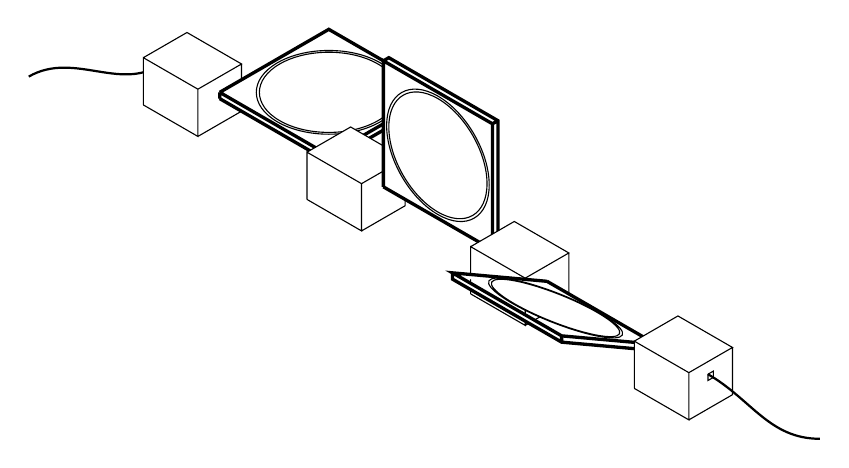
\begin{tikzpicture}[x={(0.866cm,-0.5cm)},
      y={(0.866cm,0.5cm)}, z={(0cm,1cm)}, scale=0.80]
      \tikzstyle{paddle}=[very thick, fill=white]
      \coordinate (O) at (0, 0, 0);

      % fiber in
      \draw[thick] (0,-1.5,0) to[out=30,in=220] (1,0,0);

      % first divider
      \draw[fill=white] (1,-.4,-.5) -- (2,-.4,-.5) -- (2,-.4,.25) --
        (1,-.4,.25) -- (1,-.4,-.5)
        (2,-.4,.25) -- (2,.4,.25) -- (1,.4,.25) -- (1,-.4,.25)
        (2,.4,.25) -- (2,.4,-.5) -- (2,-.4,-.5);

      % first paddle
      \draw[paddle] 
        (2,0,0) -- (4,0,0) -- (4,2,0) -- (2,2,0) -- (2,0,0) % first face
        (2,0,0) -- (2,0,-.1)
        (4,0,0) -- (4,0,-.1)
        (2,0,-.1) -- (4,0,-.1) -- (4,2,-.1);
      \draw (3,1,0) circle (.94)
        (3,1,0) circle (.9);

      % second divider
      \draw[fill=white] (4,-.4,-.5) -- (5,-.4,-.5) -- (5,-.4,.25) -- 
        (4,-.4,.25) -- (4,-.4,-.5)
        (5,-.4,.25) -- (5,.4,.25) -- (4,.4,.25) -- (4,-.4,.25)
        (5,.4,.25) -- (5,.4,-.5) -- (5,-.4,-.5);

      % second paddle
      \filldraw[paddle]
        (5,0,0) -- (7,0,0) -- (7,0,2) -- (5,0,2) -- (5,0,0) % first face
        (7,0,0) -- (7,.1,0) -- (7,.1,2) -- (5,.1,2) -- (5,0,2)
        (7,.1,2) -- (7,0,2);

      % third divider
      \draw[fill=white] (7,-.4,-.5) -- (8,-.4,-.5) -- (8,-.4,.25) --
        (7,-.4,.25) -- (7,-.4,-.5)
        (8,-.4,.25) -- (8,.4,.25) -- (7,.4,.25) -- (7,-.4,.25)
        (8,.4,.25) -- (8,.4,-.5) -- (8,-.4,-.5);

      % third paddle
      \filldraw[paddle] 
        (8,0,0) -- (10,0,0) -- (10, -1.732,1) -- (8,-1.732,1) -- (8,0,0)
        (8,-1.732,1) -- (8,-1.732,.9) -- (10,-1.732,.9) -- (10,0,-.1) -- (10,0,0)
        (10,-1.732,.9) -- (10,-1.732,1);

      % fourth divider  
      \draw[fill=white] (10,-.4,-.5) -- (11,-.4,-.5) -- (11,-.4,.25) --
        (10,-.4,.25) -- (10,-.4,-.5)
        (11,-.4,.25) -- (11,.4,.25) -- (10,.4,.25) -- (10,-.4,.25)
        (11,.4,.25) -- (11,.4,-.5) -- (11,-.4,-.5);

      \begin{scope}[x={(0.866cm,-0.5cm)},y={(0,1cm)}]
        \draw (6,0,1) circle (.94)
              (6,0,1) circle (.9);
      \end{scope}
      \begin{scope}[x={(0.866cm,-0.5cm)},y={(-.73cm,.077cm)}]
        \draw[fill=white] (9,1) circle (.94)
          (9,1) circle (.9);
      \end{scope}

      % fiber exit
      \draw (11,-.05,.05) -- (11,.05,.05) --
        (11,.05,-.05) -- (11,-.05,-.05) -- (11,-.05,.05);
      \draw[thick] (10.95,0,0) to[out=-30,in=180] (12,1,-1);
    \end{tikzpicture}
  \end{center}
\end{frame}

%
\begin{frame}[t]{Slide title {\tiny Temperature distribution}}
  \vspace*{0.10in}
  \begin{reference}{4mm}{85mm}{Black}
    \;
  \end{reference}

  \vspace*{0.10in}
  \pgfplotsset{major grid style={thin,dotted,OrangeRed}}
  \pgfplotsset{minor grid style={thin,dotted,OrangeRed!50!Black}}
  \pgfplotsset{grid style={thin,dotted,OrangeRed}}
  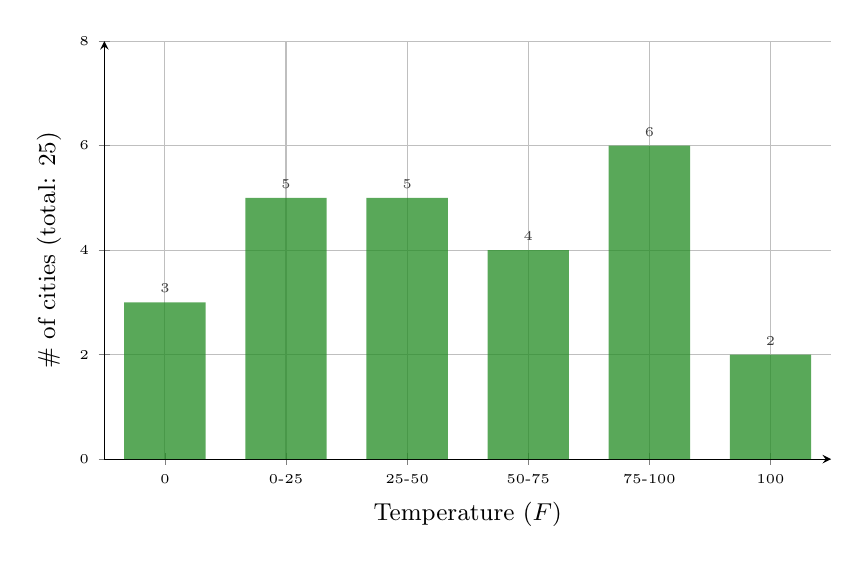
\begin{tikzpicture}[scale=0.98,font=\tiny]
    \begin{axis}[
      height=7cm,
      width=11cm,
      ybar,
      bar width=30pt,
      xlabel={\small Temperature ($F$)},
      ylabel={\small \# of cities (total: 25)},
      ymin=0,
      ymax=8,
      xtick=data,
      axis x line=bottom,
      axis y line=left,
      enlarge x limits=0.1,
      symbolic x coords={0, 0-25, 25-50, 50-75, 75-100, 100},
      grid=major,
      nodes near coords,
      legend style={draw=none,/tikz/every even column/.append style={column sep=0.5cm}}
      ]
      \addplot[draw=none,fill=ForestGreen,fill opacity=0.75] coordinates {
        (0,       3)
        (0-25,    5)
        (25-50,   5)
        (50-75,   4)
        (75-100,  6)
        (100,     2)
      };
    \end{axis}
  \end{tikzpicture}
\end{frame}

%
\begin{frame}[t]{Slide title {\tiny Temperature distribution}}
  \vspace*{0.10in}
  \begin{reference}{4mm}{85.5mm}{Black}
    25 participating cities.
  \end{reference}

  \vspace*{-0.05in}
  \begin{figure}[h]
    \def\angle{0}
    \def\radius{1.60}
    \def\labelradius{1}
    \def\cyclelist{{"ForestGreen", "Gray", "YellowGreen", "DodgerBlue", "LimeGreen", "FireBrick"}}

    \centering
    \newcount\cyclecount \cyclecount=-1
    \newcount\ind \ind=-1
    \begin{tikzpicture}[nodes = {font=\tiny},scale=2.00]
      \pgfmathsetmacro{\tcities}{25}
      %
      \pgfkeys{/pgf/number format/precision=2}
      %
      \foreach \citycount/\temprange in {
        3/0,
        5/0-25,
        5/25-50,
        4/50-75,
        6/75-100,
        2/100,
        } {
          \ifx\citycount\empty\else             % If \deptcount is empty, do nothing
            \global\advance\cyclecount by 1     % Advance cyclecount
            \global\advance\ind by 1            % Advance list index
            \ifnum6<\cyclecount                 % If cyclecount is larger than list
              \global\cyclecount=0              %   reset cyclecount and
              \global\ind=0                     %   reset list index
            \fi
            \pgfmathparse{\cyclelist[\the\ind]} % Get color from cycle list
            \edef\color{\pgfmathresult}         %   and store as \color
            %
            \pgfmathsetmacro{\percent}{\citycount*100/\tcities}
            %
            \draw[fill={\color!75},draw=none] (0,0) -- (\angle:\radius)
              arc (\angle:\angle+\percent*3.6:\radius) -- cycle;
            \draw[draw=\color!75, shorten >=3pt] (\angle+0.5*\percent*3.6:\labelradius) node {\temprange~[\citycount; \pgfmathroundtozerofill{\percent}\pgfmathresult\%]} edge (\angle+0.5*\percent*3.6:\radius);
            \pgfmathparse{\angle+\percent*3.6}  % Advance angle
            \xdef\angle{\pgfmathresult}         %   and store in \angle
          \fi
        };
    \end{tikzpicture}
  \end{figure}
\end{frame}

%
\begin{frame}[t]{Thanks be to}
  \vspace*{0.10in}
  \begin{reference}{8mm}{75mm}{Black}
    \;
  \end{reference}

  \begin{itemize}[<+->]
    \item Someone
    \item Someone
    \item Someone
    \item Someone
    \item Someone
    \item Someone
    \item Someone
  \end{itemize}
\end{frame}

% Slides end (end of edits)
%%

%
% Final slide
\finalslide

%
% Document ends
\end{document}
